\documentclass[SoftwareDesign/SoftwareDesign_main.tex]{subfiles}

\begin{document}
\section{Design av Car Profile Page}
Dette avsnittet presenterer designet av Viewet og den tilhørende ViewModelen til CarProfilePage. Den er designet med ViewFirst prinsippet på samme måte som HeaderBar.
\subsection{Design av View til Car Profile Page}
Designet for CarProfilePage er basert på en WireFrame som ble laget for siden, denne kan sees på figur \ref{fig:CarProfileWireFrame}.
\begin{figure}[H]
    \centering
    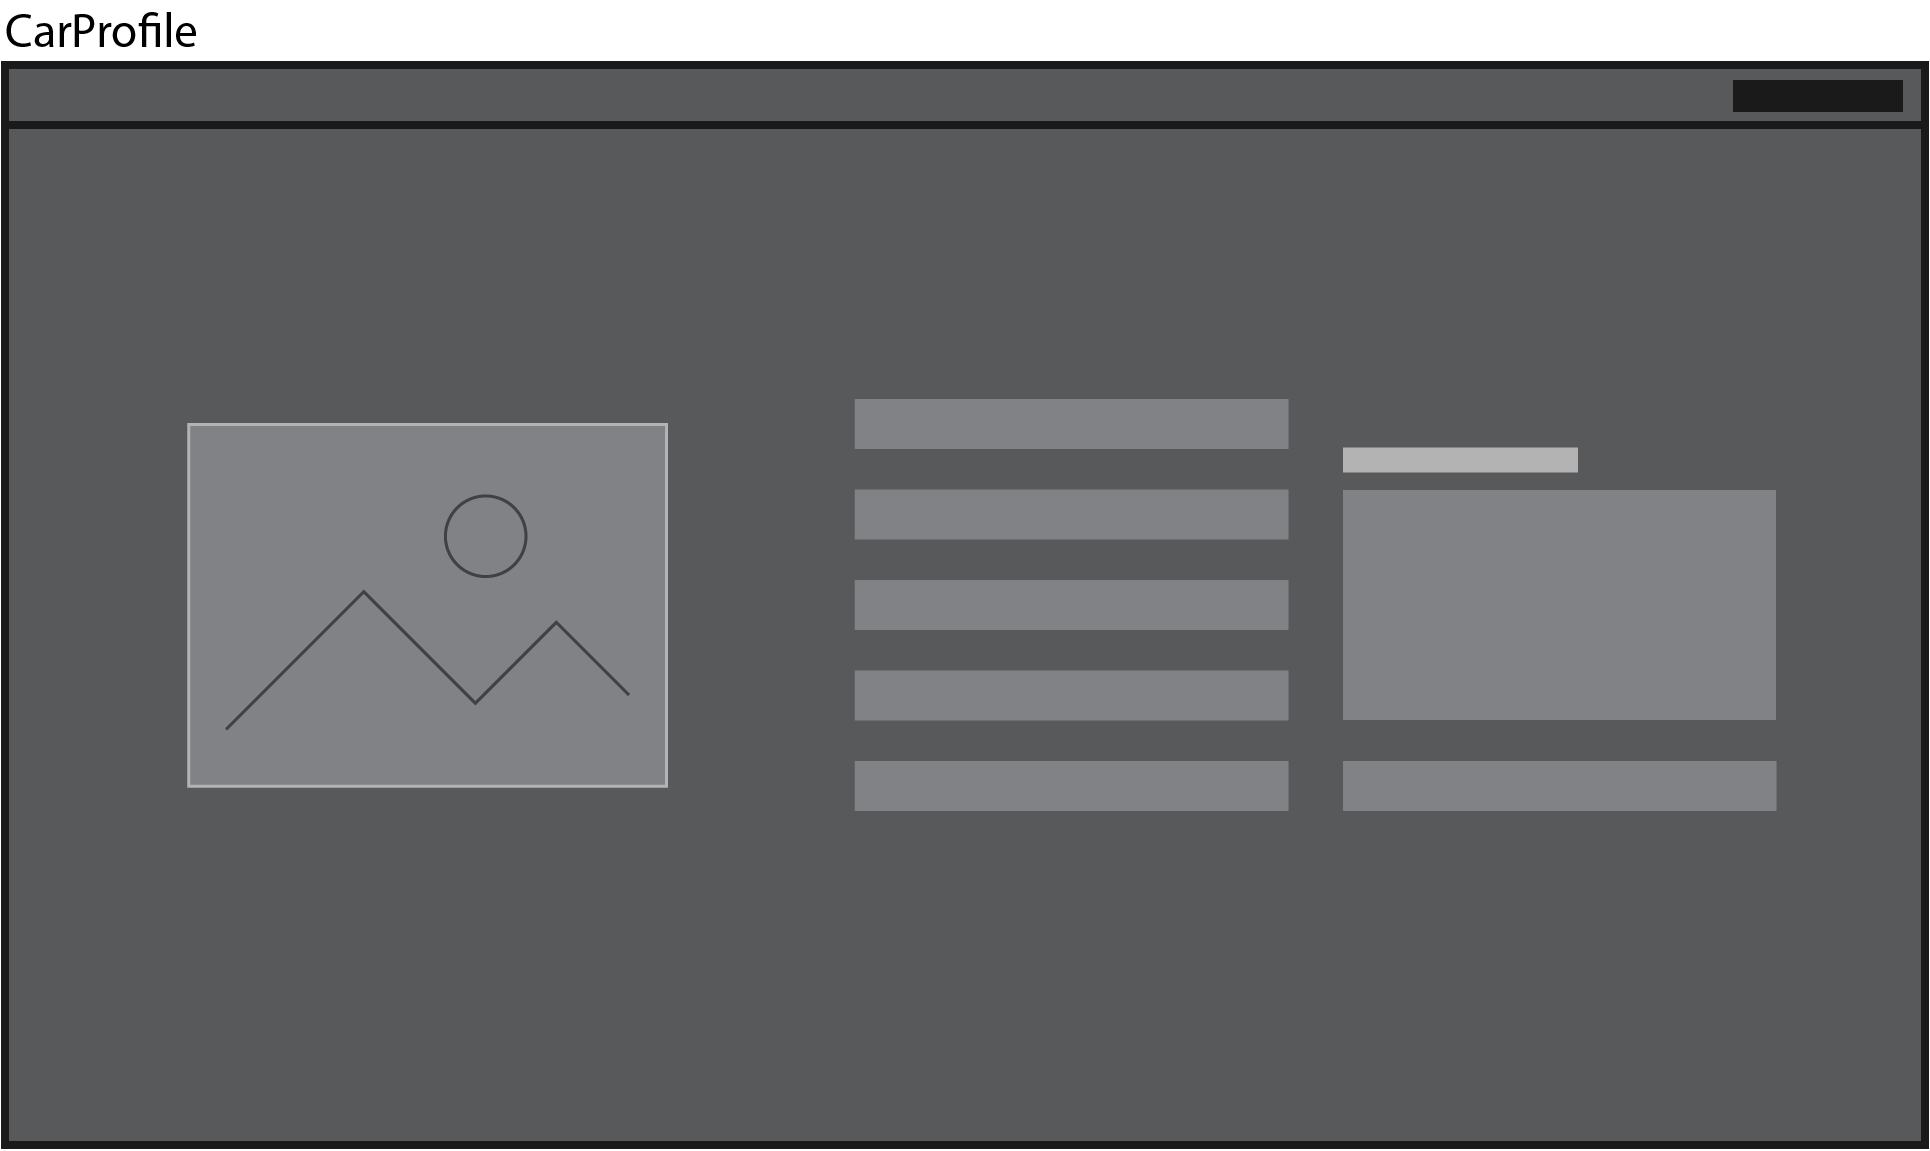
\includegraphics[width=\textwidth]{SoftwareDesign/MVVMDesigns/Graphics/CarProfileWireFrame.png}
    \caption{Car Profile WireFrame}
    \label{fig:CarProfileWireFrame}
\end{figure}

CarProfile er siden man blir tatt til når man bestemmer seg for å leie ut bilen sin derfor skal den ha flere felter hvor brukeren kan inntaste informasjonen om bilen sin blant annet merke, model og årsnummer samt et sted hvor det kan lastes opp et bilde av bilen. Dette er også siden hvor brukeren kan bestemme hviker perjoder bilen skal leies ut i. Det vil si brukeren skal kunne navigere tilbake til siden og redigere informasjonen som ligger inne om bilen.
\end{document}